\documentclass[12 pt,twocolumn]{article}
\usepackage[utf8]{inputenc}
\usepackage[spanish,mexico]{babel}
\usepackage{amsmath}
\usepackage{amssymb}
\usepackage{graphicx}
\usepackage{amsfonts}
\usepackage{float}

\begin{document}
	\title{Actividad 4}
	\author{Carolina Valenzuela Córdova}
	\date{16 de Febrero de 2016}
	\maketitle
	\newpage
	
	\section{\small Ajuste de datos por Mínimos Cuadrados}
Mínimos cuadrados es una técnica de análisis numérico enmarcada dentro de la optimización matemática, en la que, dados un conjunto de pares ordenados: variable independiente, variable dependiente, y una familia de funciones, se intenta encontrar la función continua, dentro de dicha familia, que mejor se aproxime a los datos (un "mejor ajuste"), de acuerdo con el criterio de mínimo error cuadrático.

En su forma más simple, intenta minimizar la suma de cuadrados de las diferencias en las ordenadas (llamadas residuos) entre los puntos generados por la función elegida y los correspondientes valores en los datos.\cite{w}\\
En esta actividad se nos solicitó un ajuste por mínimos cuadrados de dos colecciones de datos, y para ello fue necesario utilizar herramientas de SciPy Cookbook.

\section{\small Scipy Cookbook}
En esta página se nos proporcionó un código ejemplo con un ajuste para una función senoidal. En este código se utilizó el comando $optimize$, el cual sirve para ajustar una curva a una función a través de datos. 
\begin{verbatim}
import numpy as np
from numpy import pi, r_
import matplotlib.pyplot as plt
from scipy import optimize

# Generate data points with noise
num_points = 150
Tx = np.linspace(5., 8., num_points)
Ty = Tx

tX = 11.86*np.cos(2*pi/0.81*Tx-1.32) +
 0.64*Tx+4*((0.5-np.random.rand(num_
points))*np.exp(2*np.random.rand
(num_points)**2))
tY = -32.14*np.cos(2*np.pi/0.8*Ty-1.94) 
+ 0.15*Ty+7*
((0.5-np.random.rand(num_points)
)*np.exp(2*np.random.rand(num_points)**2))
\end{verbatim}
Como se observa, aquí fue necesario generar datos, a diferencia de que en la actividad ya se nos proporcionan dos colecciones de datos, los cuales necesitamos que nuestro programa lea y grafique de manera correcta.
\section{\small Actividades realizadas}
Para esta actividad se nos solicitó  hacer dos ajustes por medio del método de mínimos cuadrados utilizando Python, uno para cada colección de datos.
Se nos proporcionaron dos conjuntos de datos, uno referente a la temperatura en invierno de la ciudad de Nueva York, y otro de Presión atmosférica vd altitud.
En el primero se requiere realizar un ajuste lineal y en el segundo uno exponencial. A continuación se presentan los procedimientos pertinentes a cada caso:
\subsection{\small Temperatura en invierno de la ciudad de Nueva York}
Se elaboró un código similar al del ejemplo, pero con sus consideraciones para lograr que fuera lineal y leyera datos de un archivo (el que se nos dio).
\begin{verbatim}
	import numpy as np
	import matplotlib.pyplot as plt
	from scipy.optimize import curve_fit
	
	# Lee archivo de datos
	data = np.loadtxt('datos1.dat')
	
	# Guarda las columnas en los vectores
	A = data[:,0]
	T = data[:,1]
	
	# Ajuste lineal con parametros m,c
	m, c = np.polyfit(A, T, 1)
	Aajuste = data[:,0]
	
	# Evaluar xn en el ajuste calculado 
	con los param m,c
	Tajuste = np.polyval([m, c], Aajuste)
	
	# Graficar datos y ajuste
	plt.plot(data[:,0],data[:,1], 'ro')
	plt.plot(Aajuste, Tajuste)
	
	plt.show()
	\end{verbatim}
	Como se observa, tuvimos que especificar que leyera el archivo como dos columnas para que se graficara correctamente, así como especificar que fuese un ajuste lineal.También se utilizó el comando $optimize$.
	Aquí se muestra la gráfica del ajuste:
	\begin{figure}[H]
		\centering
		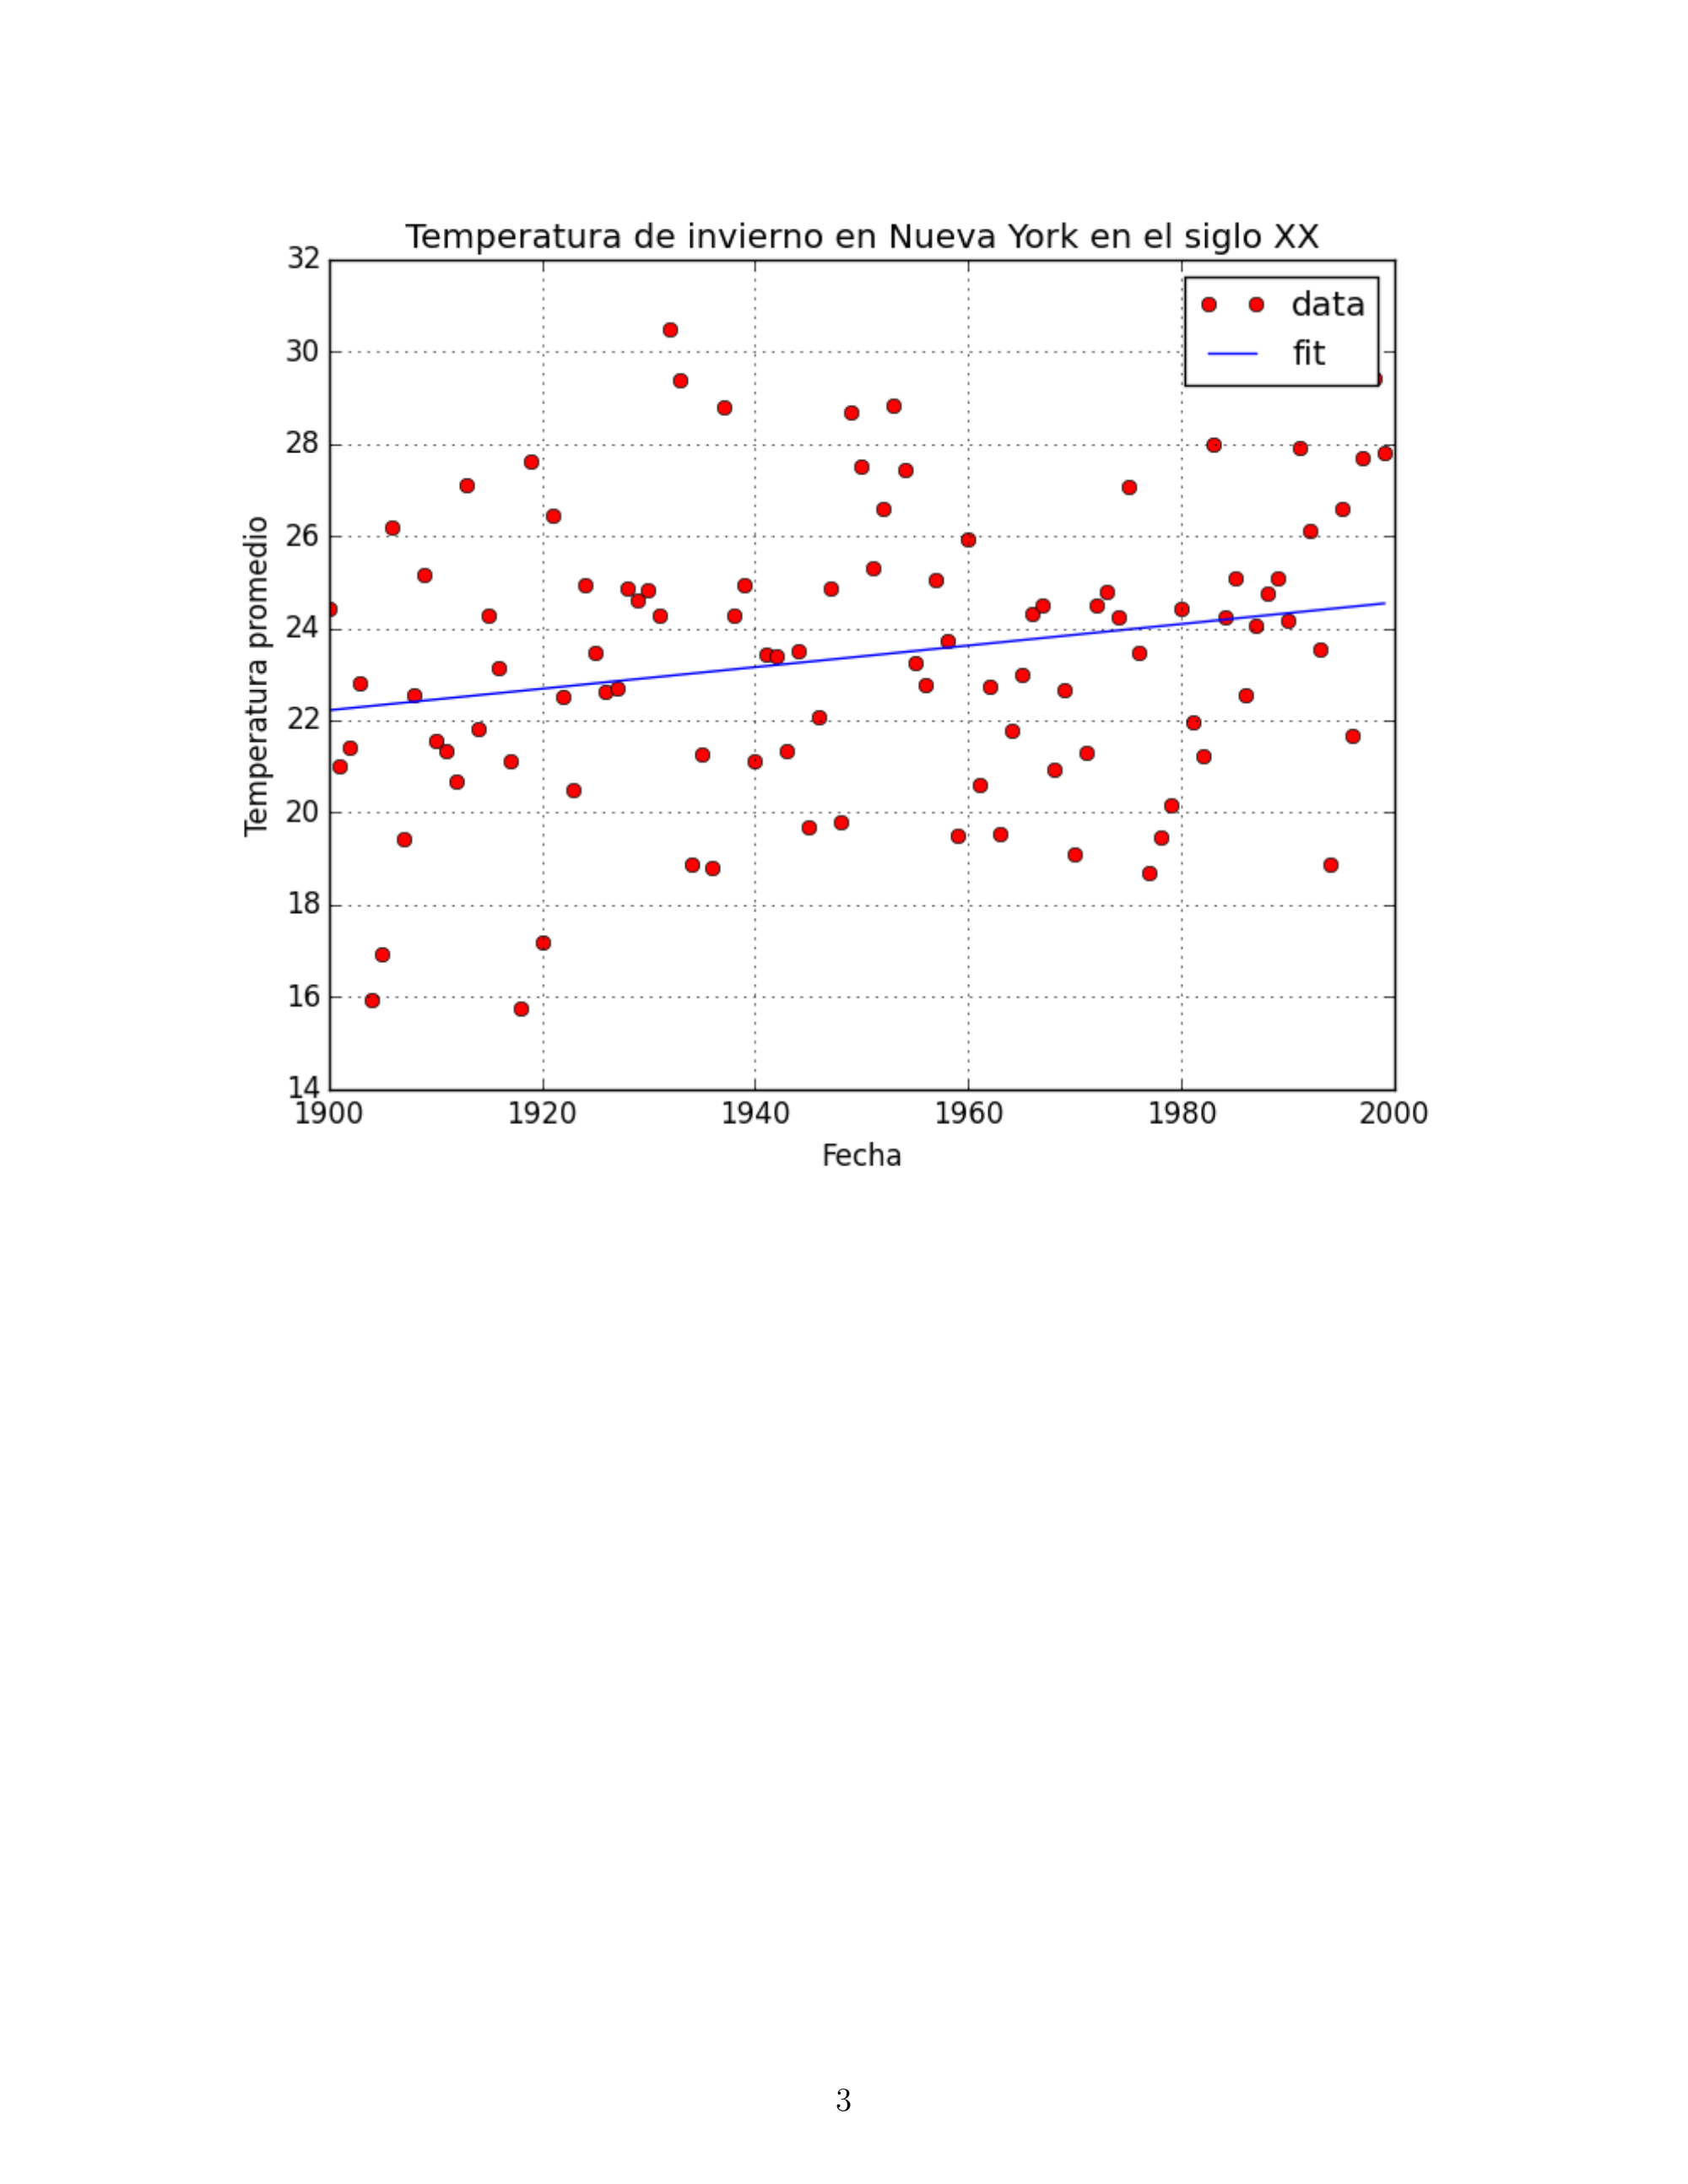
\includegraphics[width=8cm]{ajuste1.png}
		\caption{Temperatura en invierno de NYC}
	\end{figure}
	\subsection{\small Presión atmosférica vs Altitud}
	Básicamente se realizó lo mismo que para el código anterior, pero esta vez se le  especificó al programa que realizara un ajuste exponencial.
	 \begin{verbatim}
	 import numpy as np
	 import matplotlib.pyplot as plt
	 from scipy.optimize import curve_fit
	 
	 # Lee archivo de datos
	 data = np.loadtxt('datos2.dat')
	 
	 # Guarda las columnas en los vectores
	 h = data[:,0]
	 p = data[:,1]
	 h = np.array(h, dtype=float) # 
	 convertir datos a reales
	 p = np.array(p, dtype=float) 
	 
	 # Define funcion exponencial para 
	 interpolar los datos
	 def f(x, a, b, c):
	 return c * np.exp(-a * x) + b
	 
	 popt, pcov = curve_fit(f,h,p)
	 
	 # Graficar datos y ajuste
	 plt.plot(data[:,0],data[:,1], 'ro')
	 plt.plot(h, p)
	 
	 plt.show()
	 \end{verbatim}
Fue necesario incluir un arreglo que convirtiera los datos a reales dentro de la especificación de que el programa leyera el archivo en dos columnas.
Aquí se muestra la gráfica del ajuste:
	\begin{figure}[H]
		\centering
		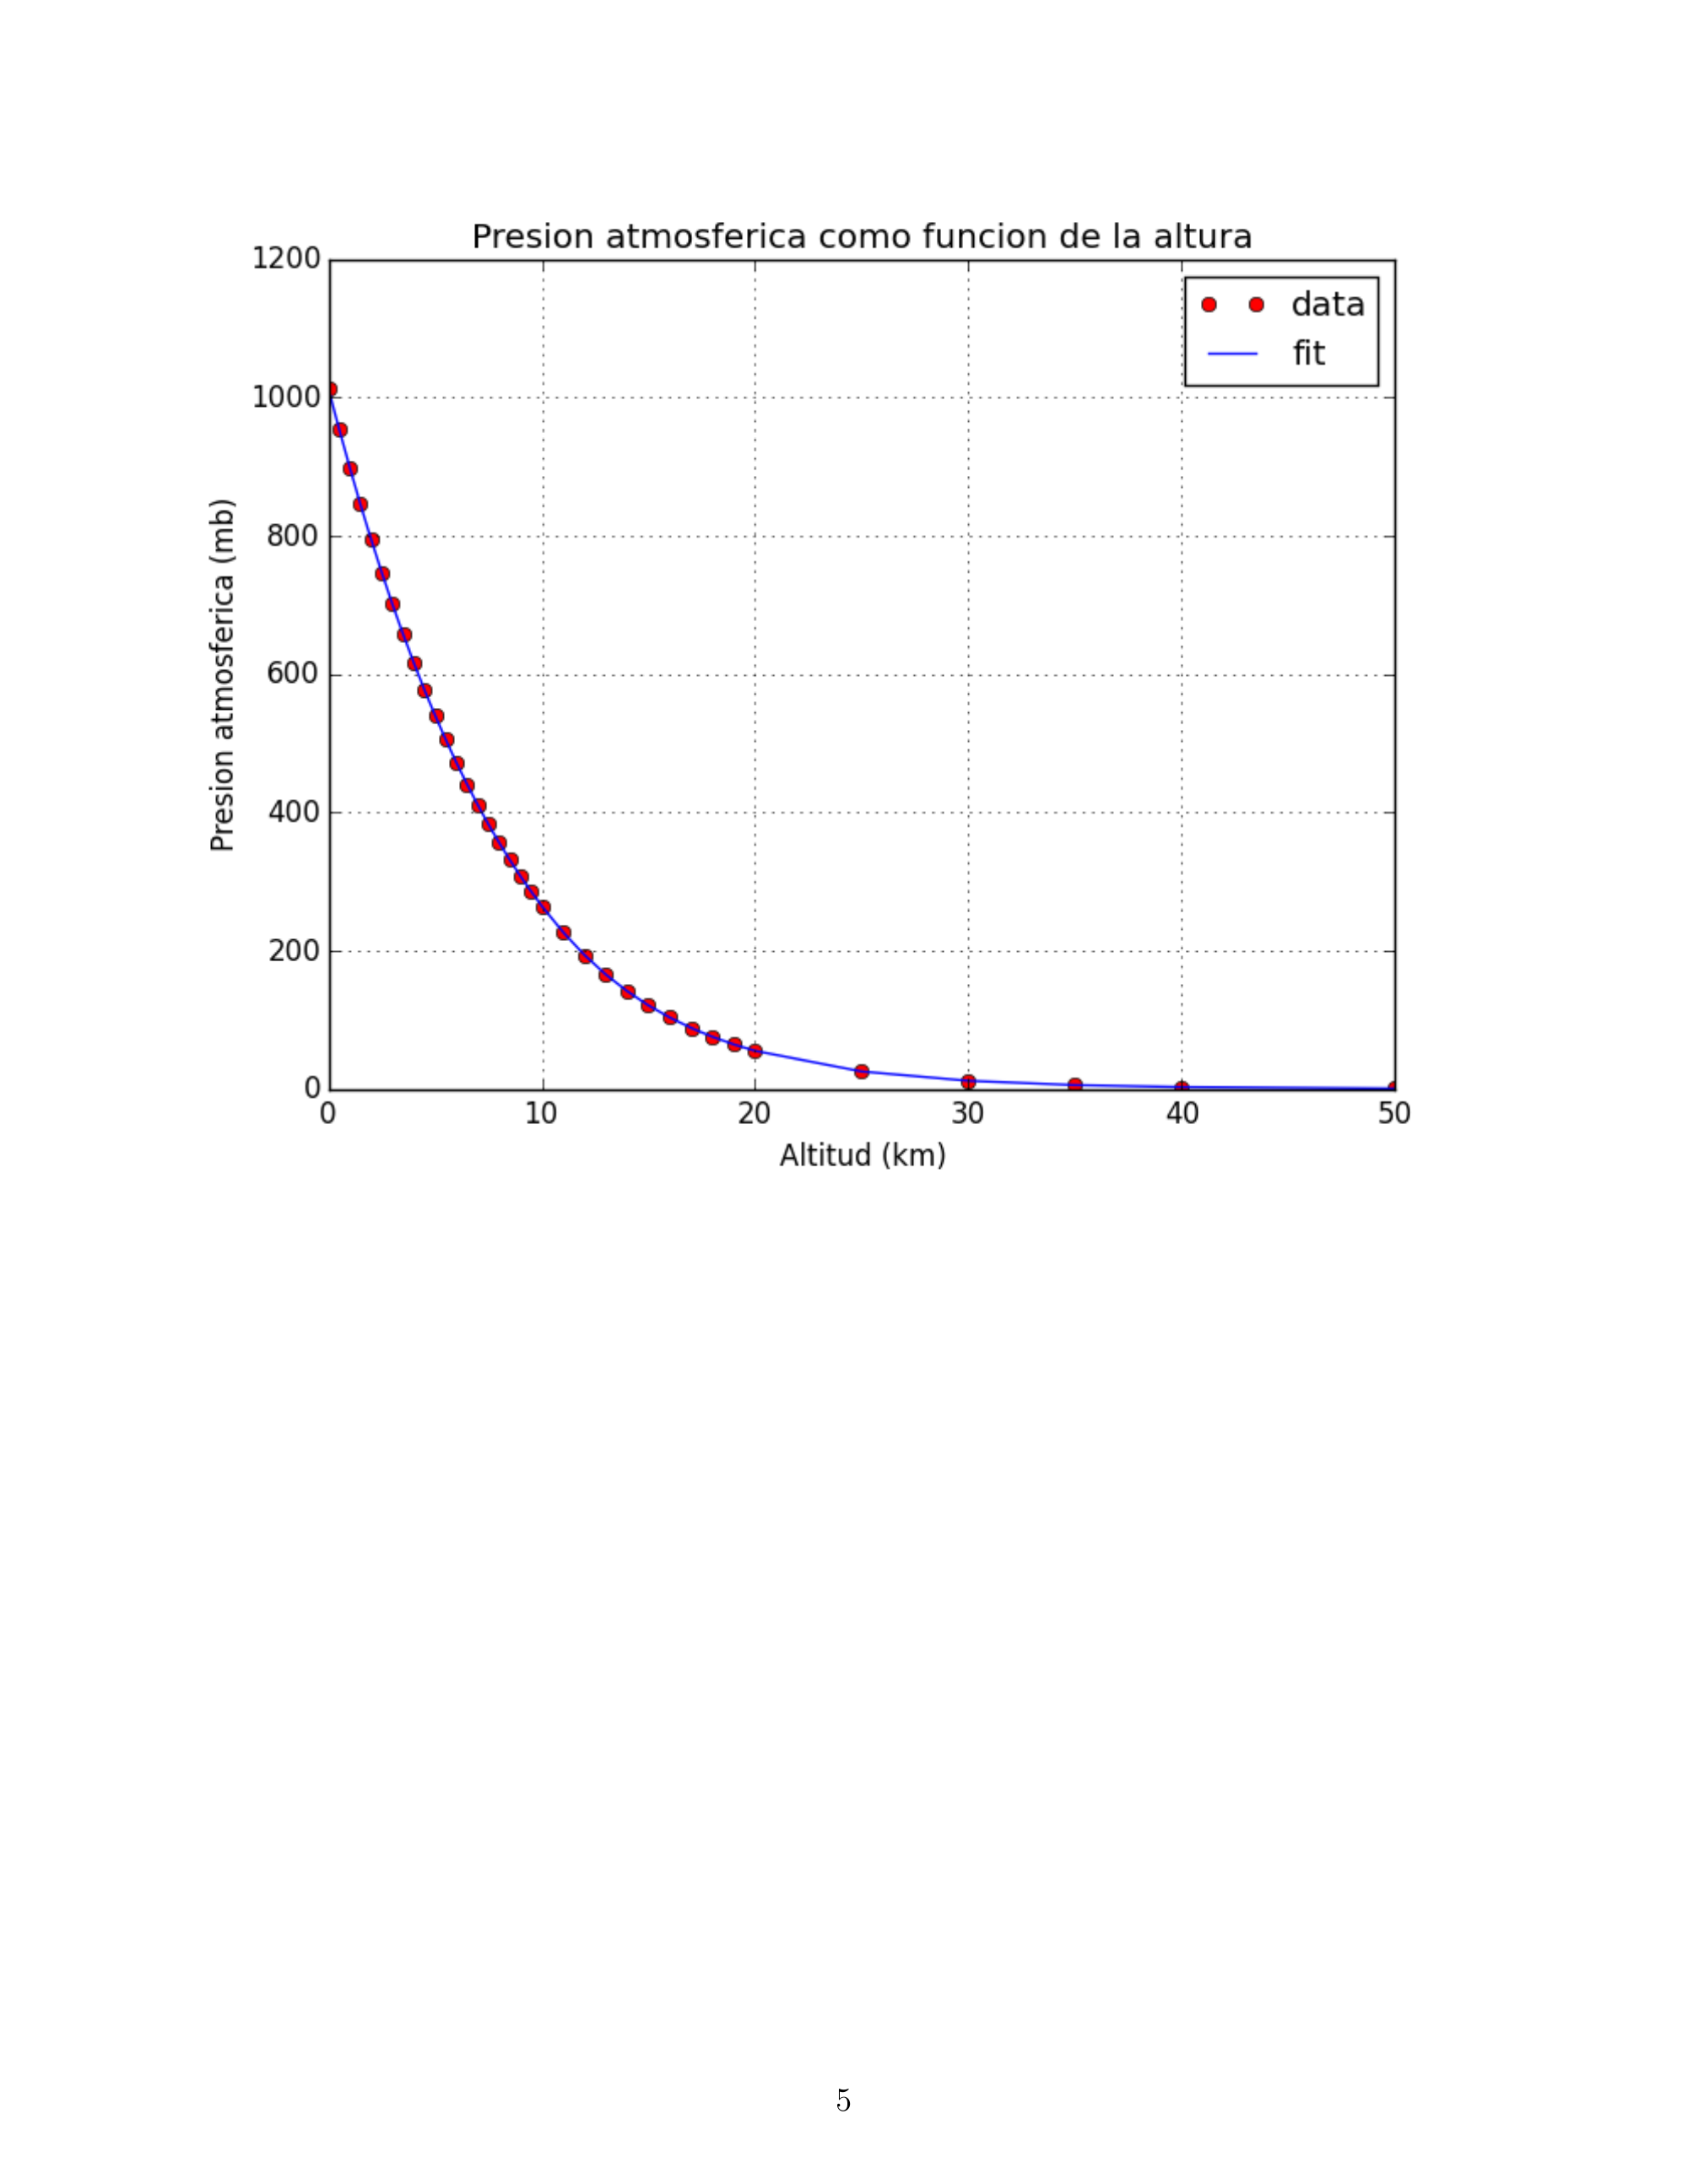
\includegraphics[width=8cm]{ajuste2.png}
		\caption{Presión atmosférica vd altitud}
	\end{figure}
\section{\small Conclusiones}
Es importante conocer herramientas computacionales que nos ayuden como físicos en proceso a en un futuro poder realizar ajustes de manera rápida y sencilla, teniendo a la mano estos programas y los manuales que se encuentran en Internet.
Este tema se vio en nuestro curso de Análisis Numérico, el cual no representó gran dificultad.

\begin{thebibliography}{widestlabel}
	\bibitem{w} Wikipedia, https://es.wikipedia.org/wiki
	/MC3ADnimoscuadrados
	
	
\end{thebibliography}
\end{document}